\chapter{Data and methods}
\label{ch:datamethods}

\section{Data}
\label{sec:data}
	\subsection{Spatial data}
		\subsubsection{Global Forest Change}
			% TODO REVIEW, CHANGE TO GOOD ENGLISH
			\ac{GFC} 2000-2012 Version 1.0 is the first high-resolution dataset that provides a comprehensive view of the annual global forest cover change between 2000 and 2012 \citep{Hansen2013, Li2017}. The initial \ac{GFC} dataset released by \citeauthor{Hansen2013} is extended by recent releases which encompass the annual forest cover changes between 2000-2013, 2000-2014, 2000-2015 and 2000-2016, respectively. All versions of this dataset have in common, that they are derived from growing season imagery captured by the remote sensing satellite Landsat 7 \ac{ETM+} enhanced by band metrics of other sensors like Quickbird imagery, existing percent tree cover layers from Landsat data, and global \ac{MODIS} percent tree cover \citep{Hansen2013}. On the satellite imagery, a time-series spectral metrics analysis is applied to gather the global forest extent at 2000 as well as the annual forest loss and the accumulated gain for the period 2001 till 2012. Hence, \ac{GFC} comprises three independent data layers tree cover, annually forest loss and forest gain divided into 10x10 degree tiles by the geodetic coordinate system \ac{WGS84} (EPSG:4326) with a spatial resolution of 1 arc-second per pixel. Furthermore, across the provided \ac{GTiff} layers the pixel data is coded in unsigned 8-bit integers. Hansen et al. defined trees as all vegetation taller than 5 meters for their study. For each pixel covered by trees, a canopy density ranging from 0 t0 100\% is computed. Forest loss is defined as a stand displacement disturbance leading from a forest state to a non-forest state (e.g. canopy density >50\% to 0\%). Tree cover gain is defined as the inverse of loss where the canopy density must exceed 50\% to get recognized.

			\note{Accuracy} % TODO ACCURACY

			The \citeauthor{Hansen2013} \ac{GFC} dataset is without any constraint publicly available for download. On the version 1.0 dataset homepage you may download "\verb|*.txt|" files containing the download \ac{URL} of the tiles for each sub dataset. The spatial location of an image tile can be determined with a tile identifier "\verb|{NAME}_{LAT}[NS]_{LNG}[WE]|" were latitude (LAT) and longitude refer to the tope left decimal corner coordinates in \ac{WGS84} and N or S as well W or E to the orientation on the hemisphere. For this project we needed the subdatasets: Treecover2000, lossyear and gain. The download process is fully automatized with an Python script by using the \ac{stdlib} modules urllib, re and threading. First this script downloads the required "\verb|*.txt|" files and creates an list where each \ac{URL} is a list element. Next it iterates over the list and extracts the corner coordinates from the file identifier with an \ac{REGEX}. This coordinate string is converted to an numeric identifier where latitude coordinates on the northern hemishpere are between $[90,0]$ and on the southern hemisphere between $(0,-90]$. Now a dataset tile is only downloaded if it is within the study extent between [30,-20] latitude. The acquired image tiles are shown in the top panel (green squares) in Figure \ref{fig:tiles}. Because we have to download in total 678 images tile the entire download process is parallized by means of multithreading.
			\begin{figure}[ht]
				\centering
				\includegraphics[scale=.96]{img/tiles}
				\caption[Map of downloaded dataset tiles]{\textbf{Map of downloaded dataset tiles:} This map shows the acquired image tiles for this study. From top to bottom in green Global Forest Change (GFC) dataset tiles (Treecover2000, lossyear and gain), the land cover dataset GlobeLand30 (GL30) image tiles in red, and in blue the Aboveground Biomass (AGB) dataset tiles. The orange filled shapes highlight countries within the tropical zone.}
				\label{fig:tiles}
			\end{figure}

		\subsubsection{GlobeLand30}
			% TODO REVIEW, CHANGE TO GOOD ENGLISH
			\ac{GL30} is the first 30 meter per pixel spatial resolution global land cover dataset that provides a comprehensive view on the distribution of 10 different land cover classes (Table \ref{tab:gl30classes}) over the earth \citep{Chen2017}. Currently this dataset is for two different time frames available 2000 and 2010 \citep{Chen2015}. The dataset is coded in unsigned 8 bit integers and as coordinates system it uses \ac{WGS84} in \ac{UTM} projection and is shipped as \ac{GTiff} in a tilled manner where each tile covers 6x5 degrees \citep{Chen2014}. For detection of the 10 land cover classes \citeauthor{Chen2015} used a so called \ac{POK} oriented approach \citep{Chen2015}. The assigned pixel values and the corresponding land cover class is listed in Table \ref{tab:gl30classes}. They grouped mapping process in different stages where each land cover type is detected separately and deleted from the source satellite image the order is: water bodies, wetland, snow and ice, cultivated land and forest, shrub land, grass land and bare land synchronous. For the detection of a land cover type they used at pixel level one of the following classifiers: \ac{DT}, \ac{SVM} or \ac{MLC}. After pixel detection they grouped the classified pixel to an object and validated this object by expert knowledge. For their approach they used satellite imagery from Landsat and HJ1 and auxiliary data like MODIS NDVI.
			\begin{table}[ht]
				\centering
				\caption[Classification schema of the GlobeLand30 product]{\textbf{Classification schema of the GlobeLand30 product:} The code column is the assigned pixel value, type the corresponding land cover type and definition explains in broad terms which types of surfaces fall into the land cover type \citep{Chen2017}.}
				\label{tab:gl30classes}
				\begin{tabular}{rlp{10.3cm}}
					\hline
					Code & Type & Definition \\\hline
					10 & Cultivated land & used for agriculture, horticulture and gardens, including paddy fields, irrigated and dry farmland, vegetable and fruit gardens, etc. \\
					20 & Forest & covered by trees, vegetation covers over 30\%, including deciduous and coniferous forest, and sparse woodland with cover 10-30\%, etc. \\
					30 & Grassland & covered by natural grass with cover over 10\%, etc.\\
					40 & Shrubland & covered by shrubs with cover over 30\%, including deciduous and evergreen shrubs, and desert steppe with cover over 10\%, etc.\\
					50 & Wetland & covered by wetland plants and water bodies, including inland marsh, lake marsh, river floodplain wetland, forest/shrub wetland, peat bogs, mangrove and salt marsh, etc.\\
					60 & Water bodies & in land area, including river, lake, reservoir, fish pond, etc.\\
					70 & Tundra & covered by lichen, moss, hardy perennial herb and shrubs in the polar regions, including shrub-, herbaceous-, wet- and barren-tundra, etc.\\
					80 & Artificial surfaces & modified by anthropogenic influence, including all kinds of habitation, industrial and mining area, transportation facilities, and interior urban green zones and water bodies, etc.\\
					90 & Bareland & with vegetation cover lower 10\%, including desert, sandy fields, Gobi, bare rocks, saline and alkaline land, etc.\\
					100 & Snow and ice & covered by permanent snow, glacier and icecap\\\hline
				\end{tabular}
			\end{table}

			% TODO ACCURACY REFERENCES GET THEM FROM CHEN2017
			\citeauthor{Chen2015} estimates an overall accuracy of 80.33\% for the product from 2010 and 78.6\% for the product from 2000 (2000 only validated at Shaanxi province in China) \citep{Chen2015}. Various scientists besides \citeauthor{Chen2015} validated the mapping accuracy of \ac{GL30} at different regions and scales. \citeauthor{Arsanjani2016} estimates an accuracy of 77.9\% for Iran and an accuracy >80\% for Germany \citep{Arsanjani2016a,Arsanjani2016}. Yang, Cao and Jacobson estimate an accuracy of 82.4\%, 80.1\% and 83.1\% for China, Nepal and East Africa, respectively \note{reference}. Unfortunately, there are no estimates for countries regions falling completely in the tropical zone.

			Chen funded the \ac{GL30} land cover mapping to the UN but it is not barrier less public available. Restriction is registration on the dataset homepage but the author was not able to register at the platform. Fortunately the supervisor of this work had already an account for this page otherwise I would be fucked. To download tiles of this dataset a order application must be filled with the required image tiles identifiers and the the year must be selected. An tile identifier "\verb|[NS]{LAT}_{LNG}|" consist of the hemisphere orientation followed by the top left corner latitude and logitude decimal coordinate (\ac{WGS84}). The homepage provides an interface for selecting the required image tiles but it is broken and buggy, especially the selection of multiple tiles did not work. Fortunately they provide a vector file which contains the dataset tile polygons with assigned identifies. This file was used to select all required tiles within the tropical zone between approxiamtely 23°N and 23°S (\ac{WGS84}), the selection is shown in red in the middle panel at Figure \ref{fig:tiles}. The corresponding identifiers were converted to an single line string and copied to application form. After submitting the form your order will be checked and approved. After one week we received 2 weeks limited access to an password protected ftp server were we downloaded the data. Due to restrictions this process of selecting data and download it could not be automatized with one pipeline only the selection and string conversion was automatized with a throw away script.\note{missing total number of tiles}

		\subsubsection{Intact Forest Landscapes}
			% TODO REVIEW, CHANGE TO GOOD ENGLISH
			\ac{IFL} 2000 is a dataset comprising a mosaic of forest and naturally treeless ecosystems without sings of human activity and large enough to maintain all native biological diversity for the time period 2000 \citep{Potapov2017}. Due to the fact that \ac{IFL} comprises different intact natural landscape patterns like primary forests, non-forest ecosystems, temporary treeless areas after a natural disturbance, and water bodies the term is not congruent to the term primary forest defined by the \ac{FAO} \citep{FAO2012}. But as mentioned \ac{IFL}s includes large patches of primary forests with a minimum extent of 500 Km$^2$ therefore primary forests can be extracted from the layer. Still there are smaller fragments of primary forest outside of the \ac{IFL}s. In regards of the extent a \ac{IFL} has a minimum size of 500 Km$^2$, a minimum width of 10 Km, and a minimum corridor/appendage width of 2 Km. Further a \ac{IFL} should not contain any of the following: ecosystem alternation, fragmentation by infrastructure and disturbance, and areas altered or managed trough agriculture, logging, and mining. For mapping and detecting \ac{IFL}s \citeauthor{Potapov2017} used Landsat imagery and several auxiliary data sources like \ac{GFC}, and national transportation maps. The dataset is may be downloaded as a \ac{SHP} with the coordinate reference system \ac{WGS84}. Each polygon in the \ac{SHP} represents an \ac{IFL} patch at an certain location on our planet.

			Data acquisition is pretty straight forward the \ac{IFL} dataset is barrier-less public available for download. As mentioned it is an \ac{SHP} so you must only download a single compressed archive. This download is realized with an Python script by using the \ac{stdlib} module urllib.

		\subsubsection{Aboveground Woody Biomass}
			% TODO REVIEW, CHANGE TO GOOD ENGLISH
			% Aboveground biomass was estimated for more than seven hundred-thousand quality-filtered Geoscience Laser Altimeter System (GLAS) lidar observations using allometric equations that estimate AGB based on lidar-derived canopy metrics. Forty-seven allometric equations were compiled from more than 20 scientific publications, with each equation developed for a different region and forest type. The most appropriate equation was determined for each shot, accounting for land cover, burned status, and Terrestrial Ecoregion of the World (TEOW) ecoregion data (Olson et al. 2001) for each shot. The equations were applied to the GLAS data, generating an AGB estimate for each shot in the global GLAS dataset. A subset of shots was classified as zero-biomass based on GLAS data and tree canopy cover and were assigned an AGB of 0 Mg ha-1.
			
			%The global set of GLAS AGB estimates was used to train random forest models that predict AGB based on spatially continuous data. The predictor datasets include Landsat 7 Enhanced Thematic Mapper Plus (ETM+) top-of-atmosphere reflectance and tree canopy cover from the Global Forest Change version 1.2 dataset (Hansen et al. 2013), 1 arc-second SRTM V3 elevation (Farr et al. 2007), GTOPO30 elevation from the U. S. Geological Survey (for latitudes greater than 60° N), and WorldClim climate data (Hijmans et al. 2005). The predictor pixel values were extracted and aggregated for each GLAS footprint in order link the GLAS AGB estimates with the predictor data. A random forest model was trained for each of six continental-scale regions: the Nearctic, Neotropic, Palearctic, Afrotropic, Tropical Asia, and Australia regions. The six regions were delineated based on aggregations of TEOW ecoregions. The predictor layers were stacked (the elevation and climate layers were resampled to match the 30-meter resolution of the Landsat inputs), and each random forest model was applied to all pixels within its region.
			
			%The data are AGB density values (megagrams biomass/hectare); aboveground carbon density values can be estimated as 50 percent of biomass density values. In addition to the AGB density map, there is an error map for an earlier version of the AGB map. This map of the uncertainty in AGB density estimation accounts for the errors from allometric equations, the LiDAR based model, and the random forest model. The error map for the current version of the biomass density map is not available yet.
			% TODO FINISH DESCRIPTION
			The \ac{AGB} raster dataset is prepared by \ac{GFW} with an adapted approach of \citeauthor{Baccini2012} \citep{Baccini2012,Baccini2015,Baccini2017}. For the year 2000, this dataset comprises the aboveground biomass density in Mg C ha$^{-1}$ (mega gram carbon per hectare) per pixel, and a confidence estimate per pixel at a spatial resolution of approximately 1 arc-second. The dataset covering the global tropical zone as an mosaic of \ac{GTiff} raster images where each tile has the \ac{CRS} \ac{WGS84} and is coded in float. For deriving biomass density \ac{GFW} used canopy metrics from \ac{GLAS} \ac{LIDAR} footprint and several allometric equations. The resulting \ac{GLAS} \ac{AGB} estimates are used to train a \ac{RF} model based on Landsat 7 \ac{ETM+}.

			The \ac{AGB} raster image tiles are public available for download on the homepage of \ac{GFW}. As mentioned before this dataset covers only the tropical zone therefore no filtering is needed before download. To receive the \ac{URL} of each image tile the \ac{GFW} homepage provides an \ac{GeoJSON} \ac{API}. The response of this \ac{API} if requested is an \ac{GeoJSON} feature collection containing the \ac{URL} of the actual biomass layer, the \ac{URL} of the uncertainty layer, and the rectangular bounds of each image tile. The data acquisition is automatized by a Python script by using the \ac{stdlib} modules urllib, threading, and the open source library Geopandas. At first the \ac{GeoJSON} is downloaded via an \ac{API} call and eventually stored on disk. Next we iterate over each feature of the \ac{GeoJSON} feature collection and extract the \ac{URL}s (biomass and confidence) of each tile. These \ac{URL}s are piped to our multi-threaded downloader and eventually store on disk. Despite mentioning the confidence layers in the dataset description, the server answers with a 404 if the confidence \ac{URL} is requested. Therefore the confidence layers are not available. In total we downloaded 105 different image tiles, there extent is shown in blue at the bottom panel of Figure \ref{fig:tiles}.

		\subsubsection{Global Soil Organic Carbon}
			The \ac{GSOCmap} is a joint project between \ac{GSP} and \ac{ITPS} to produce a global \ac{SOC} content map by a country driven approach. This year 2018, the first iteration of this map in version 1.0 was released, and later followed by 1.1 (new country submission by Rwanda) and 1.2 (new country submissions by Chile and Colombia). The mapping project is intended as a long lived dataset which will improve over time and by new country submissions. Till now 67 (approximately 63 \% of the global land mass) different countries submitted their \ac{SOC} estimates. To empower national \ac{SOC} mappings the \ac{ISRIC} provides several covariate datasets like national \ac{DEM} maps, annual spectral remote sensing data or national soil type grids. Also the contributors can join a mapping training and use the \ac{GSOCmap} cookbook as guidance for their mapping efforts. As exchange each country shares it own national \ac{GSOCmap} meeting several criteria: reporting of the Meta-data of national \ac{SOC} sampling (timeline, depth, bulk density and so on), uncertainty assessment, and the applied methods for estimating and interpolation of the \ac{SOC} content. As interpolation method the guide organizations suggest the following approaches and more: simple geo-matching, class-matching, \ac{MLR}, \ac{RF} or \ac{SVM}. The national maps are aggregated to the final \ac{GSOCmap} with a target resolution of 30 arc-seconds in the \ac{CRS} \ac{WGS84}. The dataset is one \ac{GTiff} coded in float covering the entire globe where each pixel value is the \ac{SOC} content in Mg C ha$^{-1}$ at soil depth of 0-30cm \citep{FAO2018}.

			issue border differences between countries caused by different methodologies and gap filling (if cntry dont use provided mask there is no overlap)

			Is public available as geotiff, download at fao hp, download one huge gtiff, acquisition performed by python.

		\subsubsection{Auxiliary}
			As auxiliary source for country boundaries we used the \ac{GADM} \citep{Hijmans2018}.

	\subsection{Empirical data}
		\subsubsection{Soil Organic Carbon}
			\citeauthor{Don2010} performed the first study on tropical \ac{SOC} change for soil depth between 0 and 30 cm. For the study a global meta-analysis is applied by using 358 (153 published an peer-reviewed) different studies to estimate \ac{SOC} change for 12 major \ac{LUC} types. The base date is derived from 39 different tropical countries covering all continents. Unfortunately Africa and East-Asia are under-sampled whereas South-America has the best data coverage. The meta-analysis is restricted to mineral soils therefore all wet soil types are excluded from analysis. \citeauthor{Don2010} considered 5 different \ac{LU} types for his study: primary forest, secondary forest, grassland, cropland, and perennial crops. Primary forest is defined as natural vegetation without human impacts which includes natural grassland and shrubland. Secondary forest are managed forests and regrown forest after partial destruction of the old stand. Grassland comprises pastures but excludes natural grasslands. Cropland is comprises annual crops like maize or beans and perennial crops could be coffee or sugar cane \citep{Don2010}. For our study we used only the \ac{SOC} change estimates for these \ac{LUC} types which corresponds to the \ac{GL30} and \ac{IFL} classification schema shown in Table \ref{tab:soc}.
			\begin{table}[ht]
				\centering
				\caption[Relative soil organic carbon change for certain land-use change types]{\textbf{Relative soil organic carbon change for certain land-use change types:} The Land-use change columns from and to defines the LUC type with corresponding relative Soil Organic Carbon (SOC) change and the Standard Error of the Mean (SEM) \citep{Don2010}.}
				\label{tab:soc}
				\begin{tabular}{ccrr}
					\hline
					\multicolumn{2}{c}{LUC type} & \multicolumn{2}{c}{Relative SOC change} \\
					From & To & [\%] & SEM \\\hline
					Primary forest & Grassland & -12.1 & $\pm$2.3 \\
					Primary forest & Cropland & -25.2 & $\pm$3.3 \\
					Primary forest & Secondary forest & -8.6 & $\pm$2.0 \\
					Secondary forest & Grassland & -6.4 & $\pm$2.5 \\
					Secondary forest & Cropland & -21.3 & $\pm$4.1 \\\hline
				\end{tabular}
			\end{table}

		\subsubsection{Ecosystem Service Values}


\section{Methods}
\label{sec:methods}
%TODO need more speacking section headings
%TODO flowchart
	\begin{figure}[ht]
		\centering
		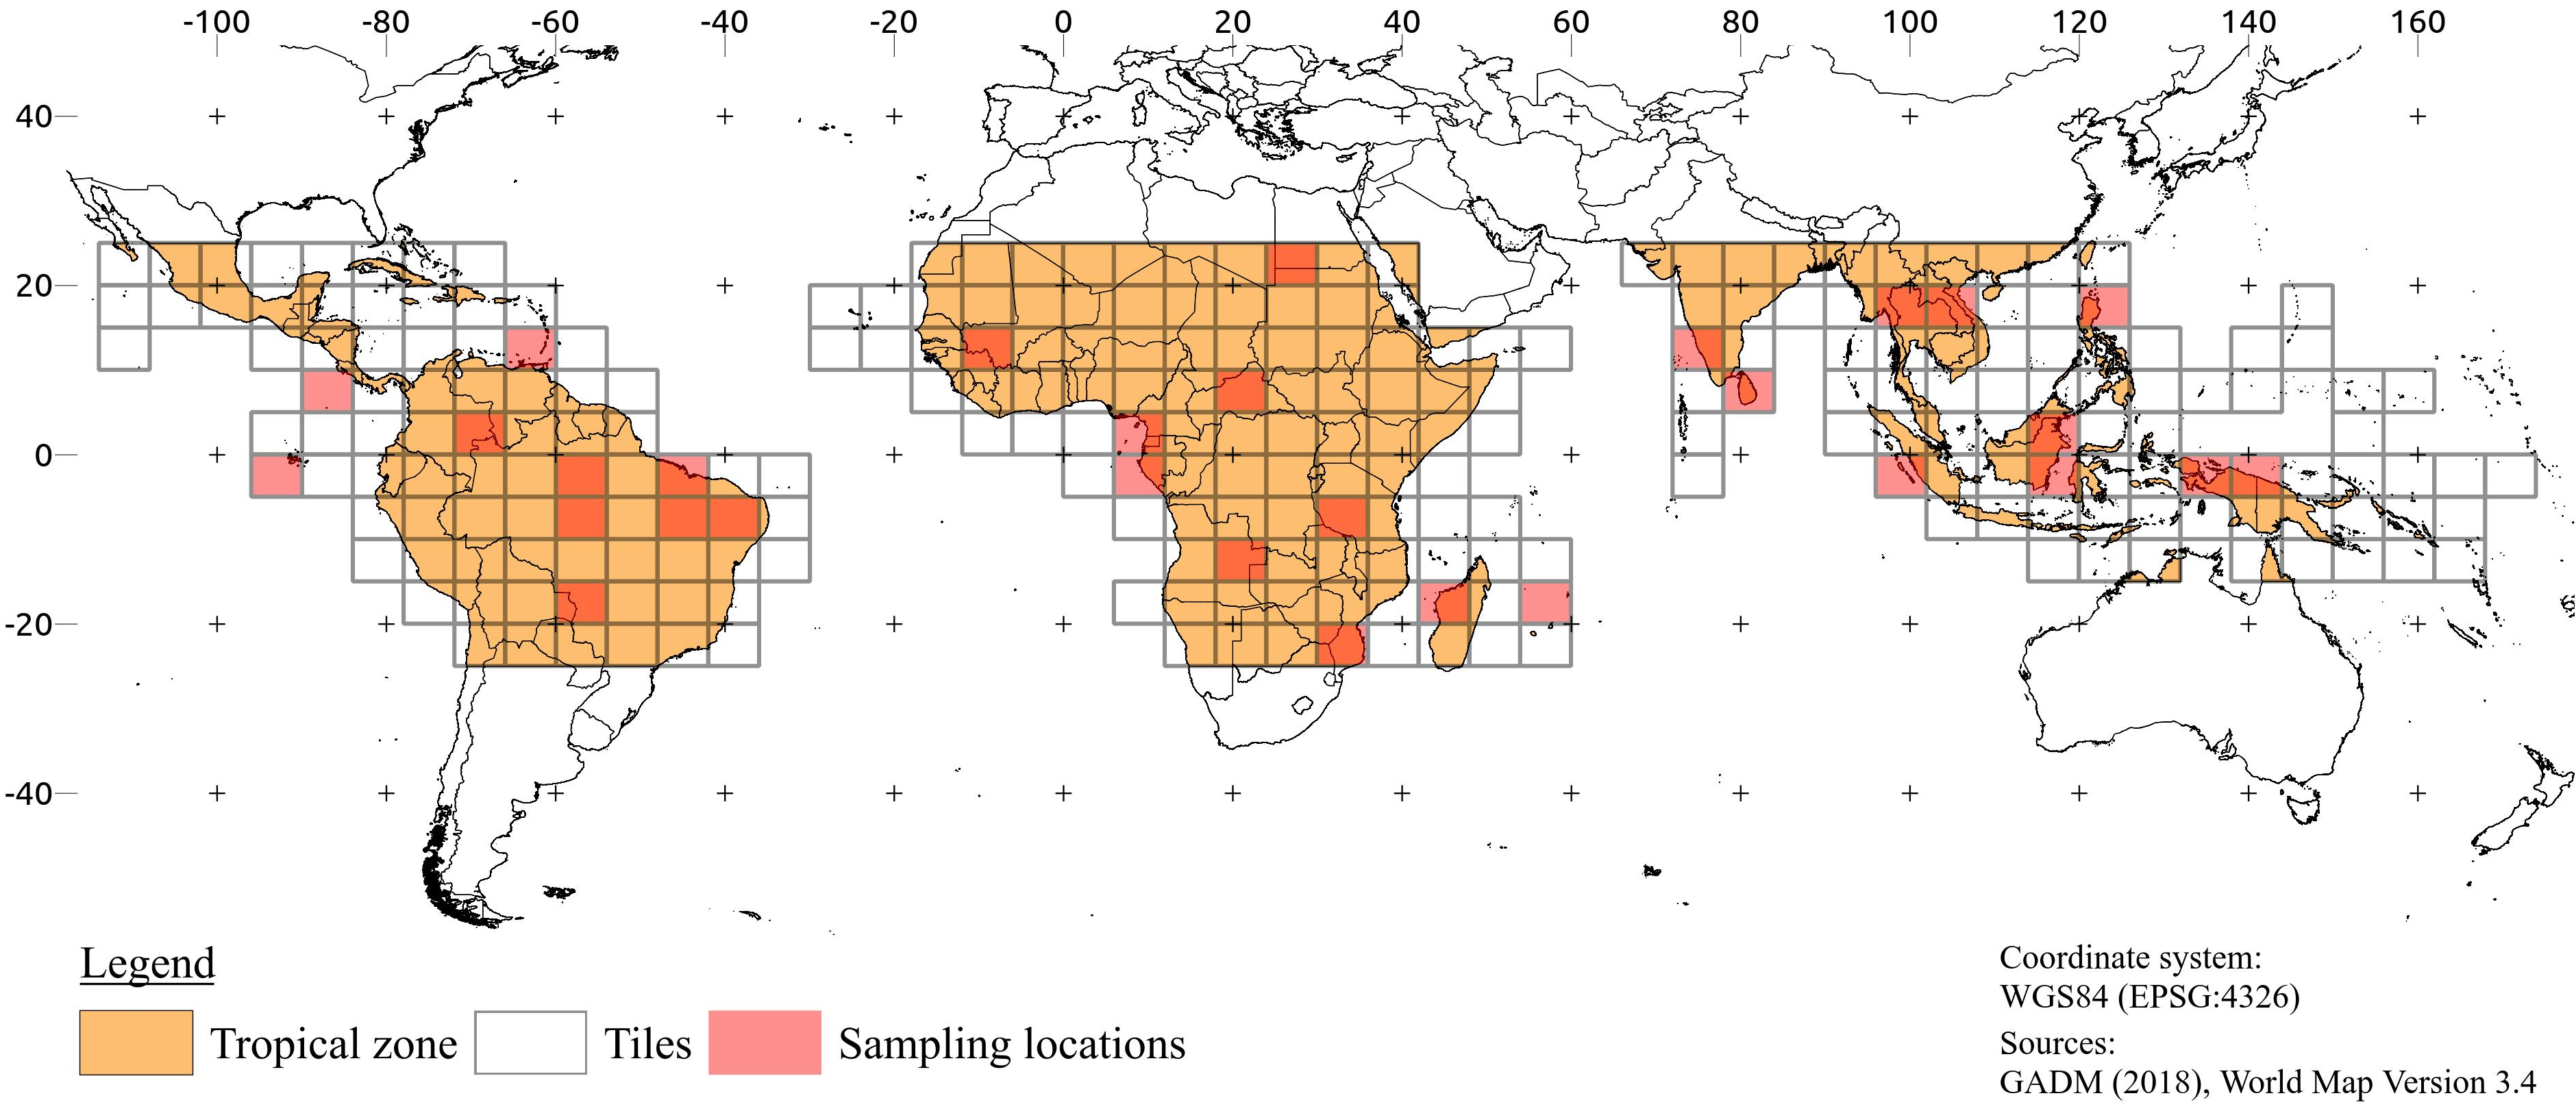
\includegraphics[scale=.97]{img/method_overview_frameless}
		\caption[Map of aligned data tiles and sampling locations]{\textbf{Map of aligned data tiles and sampling locations:} The map shows the location of the aligned multi-image stack tiles as black-framed square sized polygons, the sampling locations for accuracy assessment in red, and countries within the tropical zone in orange.}
		\label{fig:processing}
	\end{figure}

	\subsection{Pre-processing}
		Problem description, all data in different crs, also all data has diferent extent, also some data is vector data must converted to raster data. from each raster data where only tilled data set created a tile mask in target crs projection where stored name of the file an its extent. select a template datasets in our case gl30 2010. intersection compute with mask intersections are selections, now pipeline if more tiles for one needed merge them, after reproject them next clip then, for vector data to raster, software python geopandas and rasterio

	\subsection{Deforestation}
		\subsubsection{Forest definition}
			\lipsum[1-2]
		\subsubsection{Land use change driver}
			\lipsum[1-2]
		\subsubsection{Accuracy assessment}
			\lipsum[1-2]

	\subsection{Emissions}
		\subsubsection{Above ground biomass}
			\lipsum[1-2]
		\subsubsection{Soil organic carbon change}
			\lipsum[1-2]

	\subsection{Ecosystem service values}
		\subsubsection{Ecosystem service value loss}
			\lipsum[1-2]
		\subsubsection{Ecosystem service value gain}
			\lipsum[1]

	\subsection{Binning analysis}
		% TODO REVIEW, CHANGE TO GOOD ENGLISH
		The previous sections were focused on the generation of large scale spatial data. Now, a feasible method must be developed for analyzing, aggregating, interpreting and visualizing the output data. To develop a good approach we must formalize the problem domain. At first we are confronted with large N (many samples) which results in many variables (dimensionality) and complexity of relationships among this variables \citep{Carr1990}. From a visual/analytical perspective georeferenced raster maps can be interpreted as a multivariate scatter plot of large datasets where longitude and latitude represent the x and y coordinate of an data point and the pixel values (in this case nominal scaled) representing the third dimension as an group coloring. Therefore we have a large multidimensional dataset combined with a scatter plot visualization which leads commonly to over plotting issues and hidden point densities \citep{Carr1987}. Due to the spatial nature of your data we are also confronted with not equal distributed data some regions show high data densities and other regions have sparse to no data. Also a severe problem domain is the frame size of our representation. Goal is to present data on a continental level which intensifies visual problems. Each pixel has a resolution of approximately 30x30m, the continental representation of americas spanning approximately 1200000x120000km2. Therefore small scale isolated changes are hidden and only large scale changes are visual detectable. Which results in hidden details and not perceivable patterns of change.

		% TODO REFERENCE FOR MAJOR RESAMPLING APPROACH
		% TODO DESCRIBE ADVANTAGES DISADVANTAGES OF VARIOUS TESSELATIONS
		Goal should be to develop an process who solve this issues and generates satisfying output for our multivariate data. In case of raster data a re-sampling to coarser resolution could solve over plotting and resolution issues as well normalize the unequal distributed data. But the nature of re-sampling (for nominal data a nearest neighbor or majority wins \note{Reference}) would negate important spatial patterns as well frequency distributions. Another well known approach is to use binning of the spatial explicit data with a certain kind of regular polygon that is tessellating the plane \citep{Carr1992}. Polygon tessellations provide numerous opportunities for presenting multivariate statistical summaries. The scaling of the polygon could be used to represent pixel densities within the polygon area, a polygon filling color gradient is applicable to show nominal or ordinal scaled data. Also it is imaginable to use the polygon interior for a pie chart. To use regular tessellation it is important to mention there are only three types of regular polygons tessellate the plane: squares, equilateral triangles and hexagons \citep{Carr1992}. Square tessellation is the most common approach used for binning in spatial visualization. A raster image is a square tessellation. In a square mosaic each polygon shares 4 edge neighbors and 4 vertex neighbors \note{more explanation error distance disadvantages etc Hexagons properties, advantages disadvantages of both tessellations}. Final goal is to show your analysis results of spatial explicit raster data in hexagonal binned form. For bivariate maps we choose a visual representation with scaled hexagons and colorization. For multivariate details we choose a pie chart alike visualization. We split the hexagons horizontal in regards of the presented ratio. The ratios should be ordered descending so that the greatest ratio is south oriented. It is following a general description how we created the hexagon grids and how we tackled the polygon split problem. 

		% TODO REFERENCE IMAGE BETTER
		To be flexible at hexagon construction we accept 4 different parameters as construction arguments: $D$ long diagonal (Diameter of the circumscribing circle), $d$ short diagonal (diameter of the inscribed circle), $A$ area the hexagon should span and or $e$ the edge length. One selected parameter of these is used to compute $R$ the radius of the circumscribing circle with respect to input parameter as shown in  equation \ref{eq:paramters}. R is used to calculate the midpoint $<c_x, c_y>$ of the hexagon located in the first quadrant of the cartesian coordinate system Equation \ref{eq:centerx} and \ref{eq:centery}. Equation \ref{eq:hexagon} shows the computation of the hexagon anti-clockwise vertex matrix. Whereas the two leftmost vertices (first and last row of the matrix $\textbf{H}$) are located at koordinatenursprung, will sagen auf deutsch korridanten at x=0 und y=value of matrix. In summary equation \ref{eq:paramters} to \ref{eq:hexagon} show the creation of an hexagon at the leftmost corner of first quadrant (Figure \ref{fig:hexagon}). The orientation is important for the subsequent mosaic creation.
		\begin{equation}
		\label{eq:paramters}
			R = \frac{\sqrt{2A}}{\sqrt[4]{27}} = \frac{D}{2} = \frac{d}{\sqrt{3}} = e
		\end{equation}
		\begin{equation}
		\label{eq:centerx}
			c_x = \frac{R\sqrt{3}}{2} 
		\end{equation}
		\begin{equation}
		\label{eq:centery}
			c_y = R
		\end{equation}
		\begin{equation}
		\label{eq:hexagon}
			\mathbf{H} =
			\begin{bmatrix}
				0 & c_x & 2c_x & 2c_x & c_x & 0 \\
				R\sin\left(\frac{7\pi}{6}\right) + c_y & 0 & R\sin\left(\frac{11\pi}{6}\right)+c_y & R\sin\left(\frac{\pi}{6}\right)+c_y & 2R & R\sin\left(\frac{5\pi}{6}\right)+c_y \\
				1 & 1 & 1 & 1 & 1 & 1
			\end{bmatrix}
		\end{equation}
		% TODO BENCHMARK FUNCTIONS
		% TODO FINISH TESSELATION DESCRIPTION USE IMAGE
		A polygon tessellation needs several polygons to create a grid in case of the creation of one hexagon with the presented algorithm needs approximately \note{benchmark} but the creation of \note{several N hexagons} needs approximately \note{benchmark}. Therefore it is much simpler to create only one hexagon with the presented algorithm and to create the grid polygons by copying the coordinates of the source polygon and translating them to their target position with a affine transformation matrix shown in equation \ref{eq:translate}. To create the grid we get the rectangular bounds of the area to tessellate as a matrix $\textbf{B} \in R^{2\times2}$ (equation \ref{eq:bounds}), where the first column of the matrix contains the lower left corner and the second column the upper right corner of the image. Each subsequent translation in regards of $x_{off}$ is $x_1 + d$ for even rows and bla bla for odd rows. $Y_{off}$ is computed by bla bla see figure \ref{fig:hexagon}.
		\begin{equation}
		\label{eq:translate}
		\mathbf{T} =
			\begin{bmatrix}
				1 & 0 & x_{off} \\
				0 & 1 & y_{off} \\
				0 & 0 & 1
			\end{bmatrix} \circ \mathbf{H}
		\end{equation}
		\begin{equation}
		\label{eq:bounds}
			\mathbf{B} =
			\begin{bmatrix}
				x_1 & x_2 \\
				y_1 & y_2
			\end{bmatrix}
		\end{equation}
		\begin{figure}[ht]
			\centering
			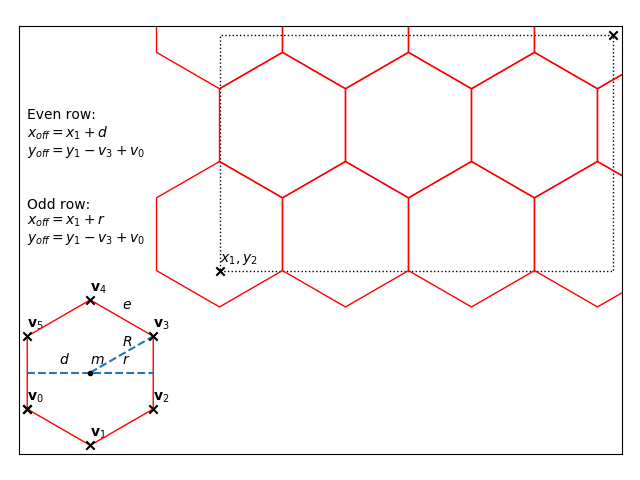
\includegraphics[scale=.7]{img/hexagons}
			\caption[Hexagon tessellation]{\textbf{Hexagon tessellation:} Located at the left bottom corner in red a hexagon defined by its geometric properties the 6 vertex vectors \{$\vec{v_0},...,\vec{v_5}$\} (black crosses), with center vector $\vec{m}$, edge length $e$, $R$ radius of the circumscribing circle, $r$ radius of the inscribed circle and $d$ the length of the short diagonal. Top right black dotted box are the bounds of an area which is tessellated by a hexagon grid in red. Each grid cell is translated from the origin hexagon at its position by computing the $x_{off}$ and $y_{off}$ offset with the presented equations at the left-hand side of the grid. }
			\label{fig:hexagon}
		\end{figure}
		% TODO DESCRIBE THE BINNING OF DATA AND WHAT WE WANT TO ACHIEVE
		Binning of raster data is easy we just have a point in polygon problem each points/pixels falling in hexagon are counted and aggregated through a function. In case of drivers of deforestation we count all driver classes per hexagon and compute ratios next we compute the sha \note{describe for each map how you build it}
		% TODO DESCRIBE CLIPPING
		As mentioned before for the visualization of the drivers of deforestation map we want to segment the hexagons with horizontal lines and each segment should represent the share of the direct deforestation driver within the tessellated area. To compute the split line for a certain hexagon we need the hexagon R computeable from the area of the hexagon equation \ref{eq:radius} and the rectangular bounds of the hexagon. We compute the relative share of an deforestation driver per hexagon this relative share can be used to compute the y-axis coordinate of an split line equation \ref{eq:percentage}. A regular hexagon can not only be presented in it vertex form as shown above. We can also use functions to define the hexagon shape. A hexagon consist of 2 picewise functions where each function consist of 3 linear functions restricted to an intervall. If we invert these functions we can use these functions to compute the x-coordinate of the split line with the previous computed y-coordinate Equations \ref{eq:left} and \ref{eq:right}. As a results we receive the solution matrix L which represents the horizontal line segment splitting the hexagon at the point where we want (driver ratio share) equation \ref{eq:line}. The solution matrix can be plugged in to a polygon split function which separates the hexagon polygon in a upper and lower part to do so we iterate over the hexagon vertices and decide if they are above or under the split line and append to a lower upper polygon. These list are our results \note{explain better split function}.
		\begin{equation}
		\label{eq:radius}
			R = \frac{\sqrt{2A}}{\sqrt[4]{27}}
		\end{equation}
		\begin{equation}
		\label{eq:percentage}
			y = \frac{P(y_2-y_1)}{100} + y_1
		\end{equation}
		\begin{equation}
		\label{eq:left}
			f^{-1}(y) =
			\begin{cases} 
				-\frac{y - y_1}{\tan{(\frac{\pi}{6}})} + \frac{x_1 + x_2}{2} & \text{if } y_1 \le y < y_1 + R\sin{(\frac{5\pi}{6})} \\
				x_1 & \text{if } y_1 + R\sin{(\frac{5\pi}{6})} \le y < R(\sin{(\frac{5\pi}{6})} + 1) \\
				\frac{y - y_2}{\tan{(\frac{\pi}{6}})} + \frac{x_1 + x_2}{2} & \text{if } R(\sin{(\frac{5\pi}{6})} + 1) \le y \le y_2
			\end{cases}
		\end{equation}
		\begin{equation}
		\label{eq:right}
			g^{-1}(y) = 
			\begin{cases} 
				\frac{y - y_1}{\tan{(\frac{\pi}{6}})} + \frac{x_1 + x_2}{2} & \text{if } y_1 \le y < y_1 + R\sin{(\frac{5\pi}{6})} \\
				x_2 & \text{if } y_1 + R\sin{(\frac{5\pi}{6})} \le y < R(\sin{(\frac{5\pi}{6})} + 1) \\
				-\frac{y - y_2}{\tan{(\frac{\pi}{6}})} + \frac{x_1 + x_2}{2} & \text{if } R(\sin{(\frac{5\pi}{6})} + 1) \le y \le y_2
			\end{cases}
		\end{equation}
		\begin{equation}
		\label{eq:line}
			\mathbf{L} =
			\begin{bmatrix}
				f^{-1}(y) & g^{-1}(y) \\
				y & y
			\end{bmatrix}
		\end{equation}
